\section{Rules}

\subsection{In brief}

\subsection{More in detail}

A decision rule is generally formed by a set of conditions and by a consequent, e.g.,
*if conditions, then consequent*. \textbf{''Given a record, a decision rule assigns to the record
the outcome specified in the consequent if the conditions are verified \cite{agrawalVLDB}``. The most
common rules are \emph{if-then rules}} that take into consideration rules with clauses in
conjunction. On the other hand, for \emph{m-of-n} rules given a set of \emph{n} conditions, if \emph{m}
of them are verified, then the consequence of the rule is applied \cite{murphyML}. When a set
of rules is used, then there are different strategies to select the outcome. For \emph{list of
rules} the order of the list is considered and the model returns the outcome of the
first rule that verifies the conditions \cite{yinICDM}. For instance, \emph{falling rule lists} are if-then rules ordered with respect to the probability of a specific outcome \cite{rudin2015}. On the other hand, \emph{decision sets} are unordered lists of rules. Basically each rule is an independent
classifier that can assign its outcome without regard for any other rules \cite{lakkaraju39}. Voting
strategies are used to select the final outcome. \marginnote{7 italic in this paragraph}[style]


List of rules and set of rules are adopted as explanation both from explanation
methods but also from transparent classifiers. In both cases the reference context is
tabular data. In \cite{augasta8} the explanation method \textsc{rxren} unveil with rules list the logic
behind a trained neural network. First, \textsc{rxren} prunes the insignificant input neurons
and identifies the data range necessary to classify the given test instance with a
specific class. Second, \textsc{rxren} generates the classification rules for each class label
exploiting the data ranges previously identified, and improve the initial list of rules
by a process that prunes and updates the rules. Figure \ref{fig:rules_rxren} shows an example of rules
returned by \textsc{rxren}. A survey on techniques extracting rules from neural networks
is \cite{Andrews4}. All the approaches in \cite{Andrews4}, including \textsc{rxren} are model-specific explainers. \marginnote{5 small caps in this paragraph}[style]

\begin{figure}[!htb]
    \centering
    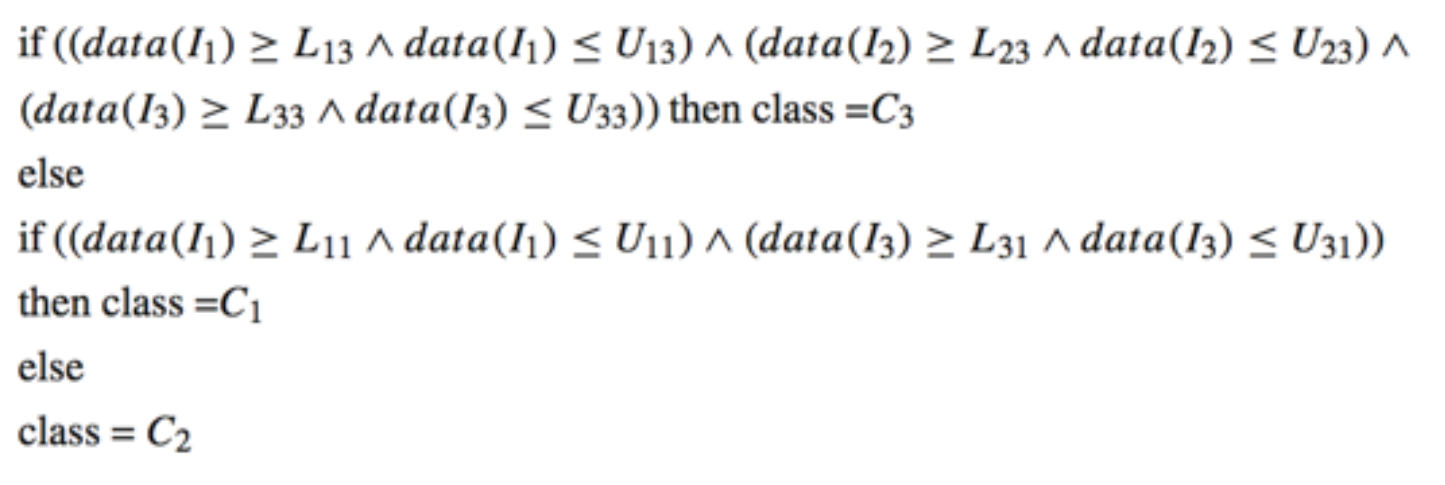
\includegraphics[width=300px]{TAILOR_T31_rules1.png}
    \caption{Example of list of rules explanation returned by \textsc{rxren}}
    \label{fig:rules_rxren}
\end{figure}


As previously mentioned, an alternative line of research to black box explanation
is the design of transparent models for the AI systems. The \textsc{corels} method \cite{angelino5} is
a technique for building rule lists for discretized tabular datasets. \textsc{corels} provides
an optimal and certifiable solution in terms of rule lists. An example of rules list
returned by \textsc{corels} is reported in Figure \ref{fig:rules_corels}. The rules are read one after the other,
and the AI would take the decision of the first rule for which the conditions are
verified. Decision sets are built by the method presented in \cite{lakkaraju39}. The if-then rules
extracted for each set are accurate, non-overlapping, and independent. Since each
rule is independently applicable, decision sets are simple, succinct, and easily to be
interpreted. A decision set is extracted by jointly maximizing the interpretability and
predictive accuracy by means of a two step approach using frequent itemset mining
and a learning method to select the rules. The method proposed in \cite{setzu63} merges local
explanation rules into a unique global weighted rule list by using a scoring system. \marginnote{3 small caps in this paragraph}[style]

\begin{figure}[!htb]
    \centering
    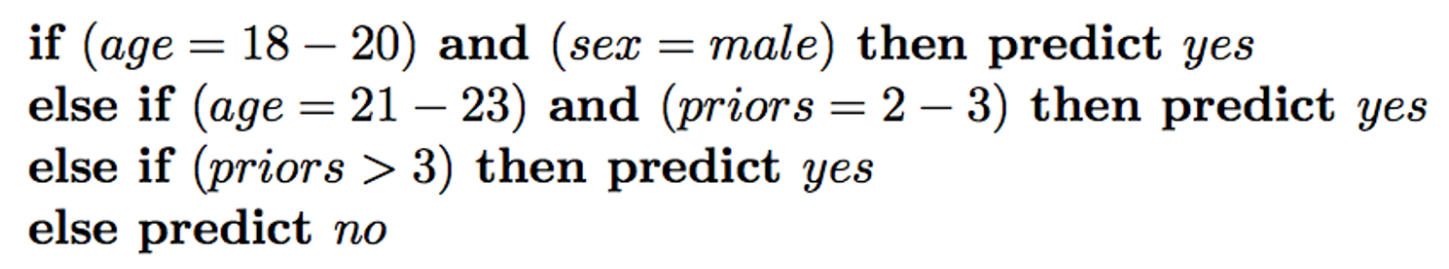
\includegraphics[width=300px]{TAILOR_T31_rules2.png}
    \caption{Example of list of rules explanation returned by \textsc{corels}}
    \label{fig:rules_corels}
\end{figure}




%```{bibliography}
%:style: unsrt
%:filter: docname in docnames
%```

> This entry was readapted from *Guidotti, Monreale, Pedreschi, Giannotti.
> Principles of Explainable Artificial Intelligence. Springer International Publish-
> ing (2021)* by Francesca Pratesi and Riccardo Guidotti.
